\documentclass[12pt]{article}
\usepackage[utf8]{inputenc}
\usepackage[a4paper, margin=1in]{geometry}
% \usepackage{pgfplots}
\usepackage{array}
\usepackage{float}
\usepackage{graphicx}
\usepackage{amssymb}
\usepackage{amsmath}
\usepackage{parskip}

\usepackage{url}
\usepackage[colorlinks,allcolors=black]{hyperref}

\usepackage{setspace}
\onehalfspacing

\setlength{\jot}{12pt} % vertical skips in equations

\title{Exploring mathematics of rolling bridges \\
    \large Extended essay \\
    \vspace{12pt} Word count: 702}

\date{}
\author{}

\begin{document}

    \maketitle
    \newpage
    \tableofcontents
    \newpage
    
    \section{Research question}

    How can catenary curves be used in construction of non-circular ``rolling'' bridges?
    
    \section{Introduction}
    
        \begin{enumerate}
            \item My personal interest - I am interested in architecture and urban planning and this topic combines this with my passion for mathematics
            \item I have found this bridge in an internet video - as an interesting mathematical phenomena existing in real life
        \end{enumerate}

        \begin{figure}[H]
            \centering
            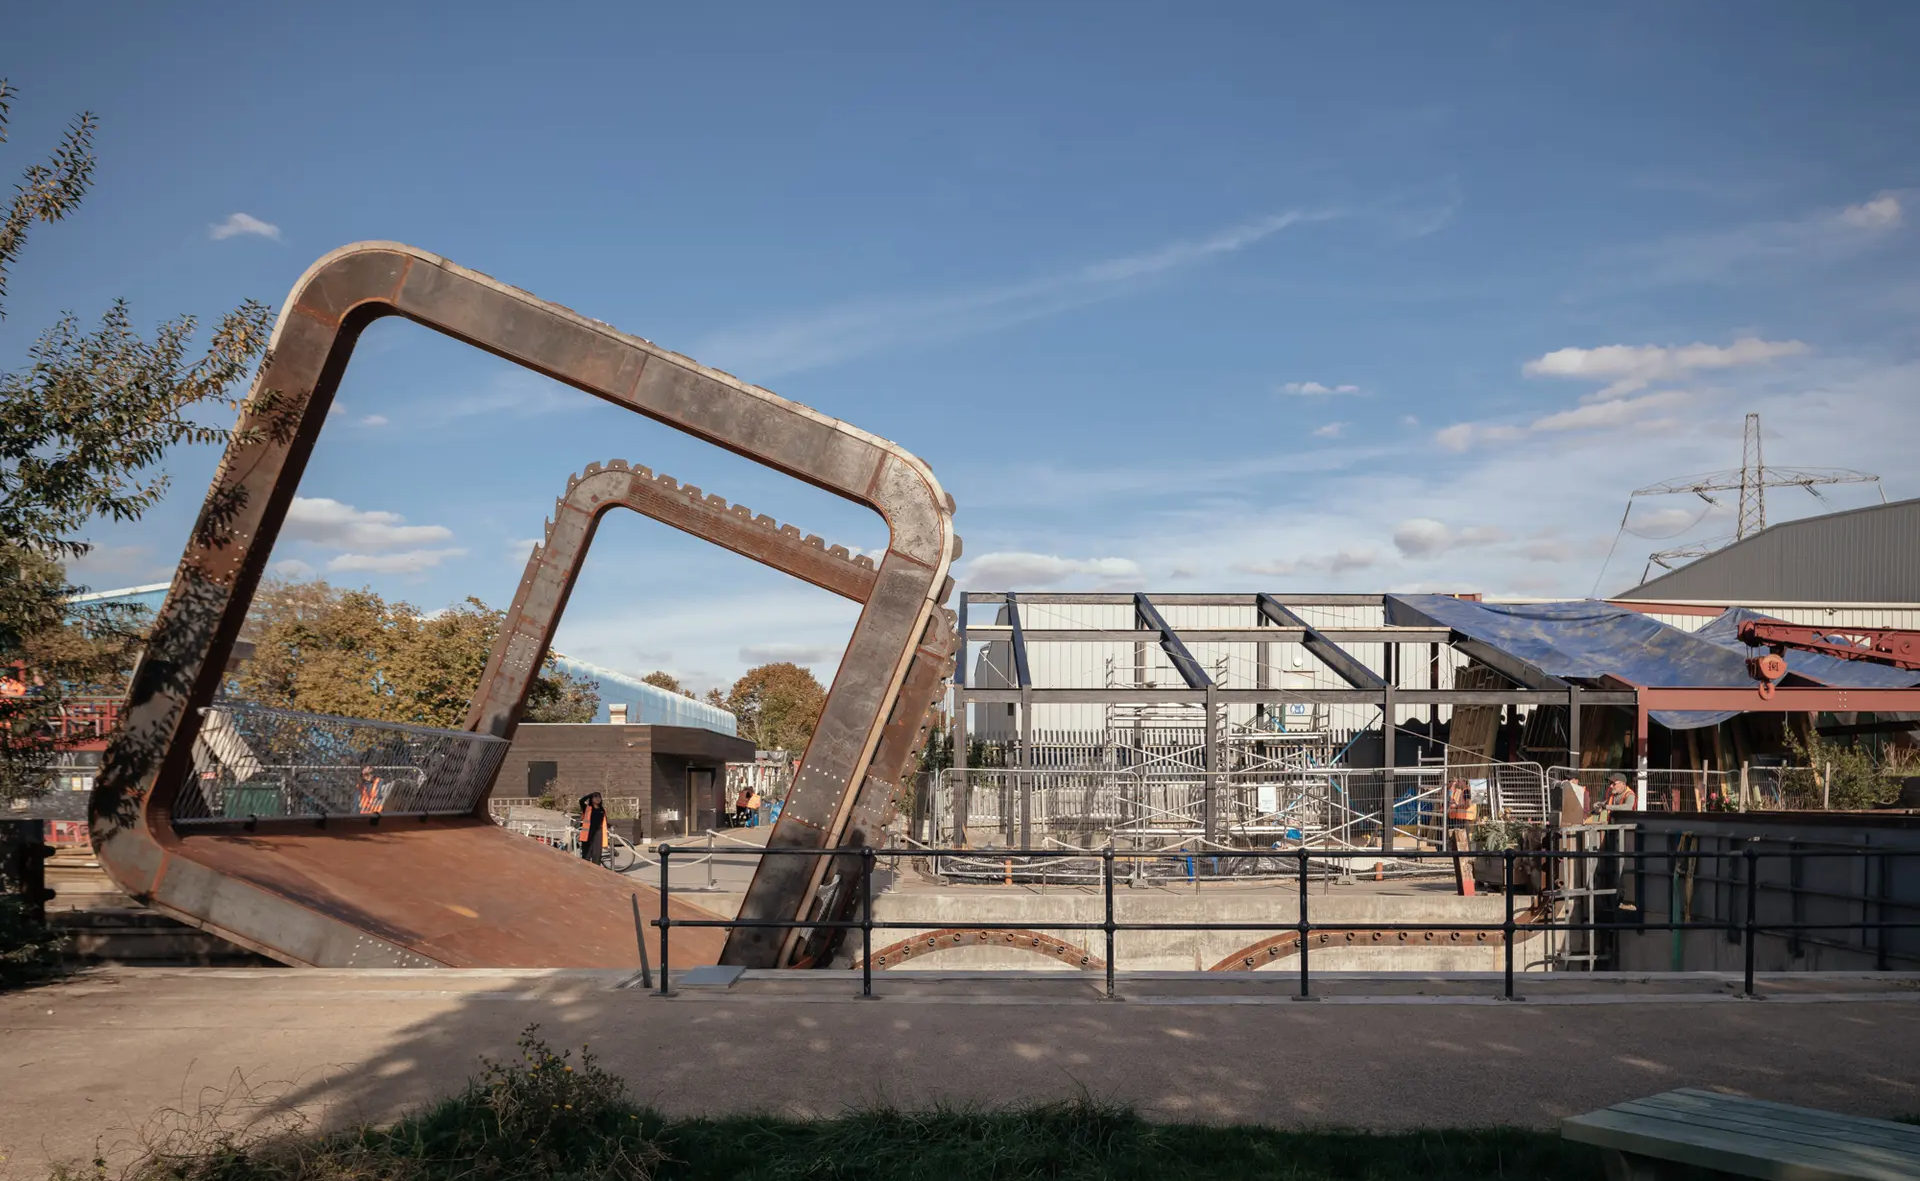
\includegraphics[width=0.75\linewidth]{images/bridge.png}
            \caption{Bridge photo \\\url{https://newatlas.com/architecture/cody-dock-rolling-bridge/}}
            \label{fig:bridge_photo}
        \end{figure}

    \section{References}

        \begin{enumerate}
            \item \url{https://community.wolfram.com/groups/-/m/t/2917199}
            \item \url{https://youtu.be/SsGEcLwjgEg}
            \item \url{https://youtu.be/xGxSTzaID3k}
        \end{enumerate}

    \newpage

    \section{Work plan}

        \begin{enumerate}
            \item square bridge \begin{enumerate}
                \item simple rolling square \begin{enumerate}
                    \item finding polar form - straight line times 4
                    \item finding relation between road and "wheel"
                    \item get y(t), then find road equation in y(x) form
                    \item catenary road = -cosh x
                \end{enumerate}
                \item rounded square \begin{enumerate}
                    \item why rounded - gears teeth
                    \item why rounded corners are hard - rolling on a circle, but centre of mass is outside of it
                    \item calculating road for the rounded square \begin{enumerate}
                        \item polar form of a rounded corner
                        \item symbolic solution \begin{itemize}
                            \item definite integration
                            \item elliptic integral of 2nd kind
                            \item cant get y(x)
                        \end{itemize}
                        \item numerical solution
                    \end{enumerate}
                    \item setting centre of mass to be at geometric centre (adding additional weight at the top of the bridge)
                    \item find location of gear teeth - roll the track around and trace intersection with bridge - inverse transformation of track around the bridge
                    \item calculating work needed to be done to roll the bridge - the centre of mass is actually 2inches below the geometric centre
                \end{enumerate}
            \end{enumerate}
            \item triangle bridge \begin{enumerate}
                \item normally cannot - too steep road and triangle crashes, but with rounded corners its possible
                \item the catenary curve is steeper, so more friction is needed
            \end{enumerate}
            \item polygonal bridge \begin{enumerate}
                \item pentagon and hexagon
            \end{enumerate}
            \item conclusion
        \end{enumerate}

    \section{``Smoothly'' rolling square}

        In order to start, the ``smooth rolling'' has to be defined. If we e.g.\ take a circle shape and roll it on a straight surface, then it will roll ``smoothly''~-~its center of mass will move only horizontally and not vertically. However, when a square is rolled on the same surface, its center of mass will move vertically as well and hence its movement will not be ``smooth''.

        Even so, why is it important to roll ``smoothly''? The answer is connected to physics, more specifically to the work needed to be done to roll the shape. If the figure is rolled ``smoothly'', then there is no need to do work in moving the center of mass up and down. Therefore, in the ideal world, the shape will roll without any work needed to be done (in reality, there is always some friction, so some work will always be needed to be done).

        Another important property for this ``rolling'' is that when any point of the shape is in contact with the road surface, its velocity relative to it has to be zero. Otherwise, if the point was moving while touching the road, it would be sliding and not rolling.

        However, there must exist a surface (other than straight road) on which a square can roll ``smoothly''. It will be described parametrically as follows:
        \begin{align}
            \begin{cases}
            x = x(t) \\
            y = y(t)
            \end{cases}
        \end{align}

        Similarly, the square shape will also be parametrized. However, it will be parametrized in polar coordinates, as this representation will be easier to work with. The parametrization is as follows: 
        \begin{align}
            \begin{cases}
            r = r(t) \\
            \theta = \theta(t)
            \end{cases}
        \end{align}

        To simplify the calculations, the line of movement of the center of mass of the square will be chosen to be the x-axis. Hence, the road will have to be under it, so $y(t) < 0$. Likewise, the center of mass of the square point (axle) will be chosen to be at the origin of its local coordinate system. The parameter $t$ can be thought of as the time, at which there is a point on the square and on the road, which are touching. Therefore, the point $(x, y)$ on the road will be the contact point on the road curve and similarly the point $(r, \theta)$ will be the contact point on the square curve.

        Now, the relations between those two curves need to be found. If it is assumed that the square is on the road, then it must be touching it at some point. Moreover, the point of contact is not a random point on the curve, but the one directly beneath the center mass point (so the origin point). Therefore, it has to be the $r(t)$ point on the square curve. Hence, the distance from axle to the road must be equal to the road's depth ($-y(t)$):
        \begin{equation}
            r(t) = - y(t)
        \end{equation}

        Another relation can be found by looking at the contact point's velocity. It was earlier defined, that during contact, the velocity of a point relative to the road has to be zero. However, when it is looked at from the perspective of the axle point, all points on the square are constantly moving (while rolling). Therefore, if the point is stationary relative to the ground, but moving relative to the center point, then those speeds have to be equal to each other. The speed relative to road is simply $|\frac{dx}{dt}|$, while the speed relative to the axle can be calculated from its angular speed:
        \begin{flalign*}
            \omega &= \frac{d\theta}{dt} \\
            v &= r \cdot \omega \\
            v_{\text{axle}} &= r \frac{d\theta}{dt}
        \end{flalign*}

        Thence (the speeds, not the velocities are equal, hence the absolute value):
        \begin{align}
            \bigl|\frac{dx}{dt}\bigr| = \bigl|r \frac{d\theta}{dt}\bigr| \nonumber \\
            \frac{dx}{dt} = \pm\; r \frac{d\theta}{dt}
        \end{align}

        However, it can be assumed that the square will roll to the right (in the positive $x$ direction), so the contact point will have to rotate counter-clockwise. Therefore, both $\frac{dx}{dt}$ and $\frac{d\theta}{dt}$ have to be positive. Hence:
        \begin{equation}
            \frac{dx}{dt} = r \frac{d\theta}{dt}
        \end{equation}

        Therefore, there are two relations between the road and square curve:
        \begin{equation}
            \begin{cases}
                r = - y \\
                \frac{dx}{dt} = r \frac{d\theta}{dt}
            \end{cases}
        \end{equation}

        The $y$ part of the road curve can easily be found:
        \begin{align}
            % r(t) = - y(t) \nonumber \\
            y = -r
        \end{align}

        For the $x$ part:
        \begin{flalign}
            \frac{dx}{dt} &= r \frac{d\theta}{dt} \nonumber\\
            \int \frac{dx}{dt} dt &= \int r \frac{d\theta}{dt} \;dt \nonumber\\
            \int dx &= \int r \;d\theta \nonumber\\
            x &= r\theta + c
        \end{flalign}

        Hence:
        \begin{equation}\label{eq:road_1}
            \begin{cases}
                y = -r \\
                x = r\theta + c
            \end{cases}
        \end{equation}

        Now, the parametric functions for a square need to be found in order to find the road curve. For the simplicity of this calculation let the side length of the square be 2. To find the equations it is easiest to start with just a single side of the square (starting at $(1, -1)$ and ending at $(1, 1)$). Therefore:
        \begin{align}
            x(t) = 1 \\
            y(t) = t
        \end{align}

        Those formulas can be converted to polar form using the following equations\cite{polar_rectangular}:
        \begin{align}
            r &= \sqrt{x^2 + y^2} \\
            \theta &= \arctan\frac{y}{x}
        \end{align}

        Therefore:
        \begin{align}
            r(t) &= \sqrt{1^2 + t^2} = \sqrt{1+t^2} \\
            \theta(t) &= \arctan\frac{t}{1} = \arctan(t)
        \end{align}

        These equations may be used to substitute into Equation \ref{eq:road_1}:
        \begin{align}
            y &= -r = -\sqrt{1+t^2} \\
            x &= r\theta + c = \sqrt{1+t^2}\arctan(t) + c
        \end{align}

        Therefore:
        \begin{equation}\label{eq:road_2}
            \begin{cases}
                x(t) = \sqrt{1+t^2}\arctan(t) + c \\
                y(t) = -\sqrt{1+t^2} \\
            \end{cases}
        \end{equation}

    % bibliography
    \newpage
    \bibliographystyle{unsrt}
    \bibliography{refs}

    % \section{Conclusion}
    
    %     \subsection{Reflections}    
    
    %     \subsection{Limitations}
    
    %         How to improve, etc.
        
\end{document}
